\subsection{Compiler un document avec bfcours}

\begin{Methode}[Première compilation avec bfcours]

    L'architecture recommandée pour éditer des documents \LaTeX\ est la suivante : 
    \begin{tcbraster}[raster columns=3,blank]
        \begin{tcolorbox}[blank,raster multicolumn=2]
            \dirtree{%
                .1 \textbf{NomPrincipal}.
                .2 \textcolor{blue}{images/}\DTcomment{Dossier pour toutes les images}.
                .2 \textcolor{blue}{sections/}\DTcomment{Optionnel pour les gros fichiers}.
                .2 \textcolor{blue}{annexes/}\DTcomment{Optionnel, documents auxiliaires}.
                .3 scripts/.
                .3 csv/.
                .3 todolists/.
                .2 \textbf{NomPrincipal.tex}\DTcomment{Fichier principal à compiler}.
                .2 enonce.tex\DTcomment{Contenu principal, organise les sous-fichiers}.
                .2 enonce\_figures.tex\DTcomment{Contient les figures TikZ du projet}.
            }

            Les répertoires en \encadrer{bleu} sont présents en cas de nécessité seulement.
        \end{tcolorbox}
        \begin{tcolorbox}[blank] 
            Cette organisation permet de :
            \begin{itemize}[label=$\bullet$]
                \item Séparer clairement le contenu de la structure : les en-têtes sont dans le \acc{fichier principal} et le contenu est dans \acc{enonce.tex}.
                \item Produire différentes versions pour un même contenu ( A3, dys, corrections, élève... )
                \item Faciliter la maintenance et les modifications
                \item Réutiliser des éléments entre différents projets
            \end{itemize}
        \end{tcolorbox}
    \end{tcbraster}


    Pour \voc{compiler} un document \LaTeX\ avec bfcours, il suffit de : 
    \begin{tcbenumerate}
        \tcbitem \tcbitempoint{1} \'Ecrire le contenu dans un fichier nommé \acc{enonce.tex}
        \tcbitem \tcbitempoint{1} Compiler le \acc{fichier principal} en utilisant \acc{LuaLaTeX} - sinon ça ne compile pas. 
    \end{tcbenumerate}
\begin{Remarque}
    LuaLaTeX est un compilateur permettant de compiler avec le moteur \LaTeX\ tout en autorisant l'utilisation de scripts écrits en langage Lua. 

    Ce langage est simple et fonctionne sur tous les hardware, mais n'est pas autorisé par défaut dans les compilateurs \LaTeX.
\end{Remarque}
\end{Methode}

\begin{EXO}{Première compilation avec bfcours}{BF-1}

    \itempoint{1}Accéder au répertoire \displayFilePath{fichiers\_de\_la\_formation/2.Exercices\_bfcours}.

    \itempoint{1}Ouvrir son fichier principal \displayFilePath{fichiers\_de\_la\_formation/1.Exercices\_bfcours/Exercices\_bfcours.tex} avec \acc{VScode} ( ou l'\voc{IDE} de votre choix ).

    \itempoint{1}Compiler le fichier.
    
    \exocorrection

    Il faut compiler avec \acc{LuaLaTeX}.
\end{EXO}
\subsection{Utiliser les environnements didactiques}

\begin{MultiColonnes}{2}
    \tcbitem Le package \bfcours\ propose des \acc{environnements didactiques} destinés à la transmission de connaissances. 

    Ils s'utilisent de manière très simple mais agissent à plusieurs niveau et sont l'aboutissement de beaucoup de travail.
    \tcbitem \begin{itemize}[label=$\bullet$]
    \item Présentation claire isolant le contenu du reste du document. 
    \item Insertion dans la table des matières. 
    \item Gestion des couleurs permettant une cohérence visuelle.
    \item Gestion des marges et de la police.
    \item Pour les exercices : gestion des numéros, des corrections séparées, des points et de la difficulté.
\end{itemize}
\end{MultiColonnes}
\begin{tcolorbox}[blank]
    \begin{tcbenumerate}[2]
        \tcbitem \tcbitempoint{1} On peut donc utiliser tous les environnements suivants librement, via la syntaxe :

            \showenv[blue]{NomEnvironnement}[[titre][options]]

            \begin{itemize}[label=$\bullet$]
                \item \textbf{NomEnvironnement} : Le nom de l'environnement commence toujours par une majuscule et sans accent (Exemple : \texttt{Methode}, \texttt{Definition}, \texttt{Theoreme}).
                
                \item \textbf{Titre} : La première option correspond au titre.
                
                \item \acc{Options} : La seconde option est destinée à ajouter des options tcolorbox dans la définition de l'environnement.  
            \end{itemize}
            \begin{Remarque}
                L'environnement \acc{EXO} a une syntaxe particulière :
            
                \showenv[red]{EXO}[\{Titre\}\{Code compétence\}]
                
            \end{Remarque}
        \tcbitem[valign=top] \tcbitempoint{1}Environnements didactiques
        
        \begin{tcbtab}{p{0.24\textwidth}p{0.54\textwidth}}%

                \textcolor{meth}{\textbf{Methode}} & Pour présenter des méthodes de résolution \\
                \textcolor{defi}{\textbf{Definition}} & Pour introduire une nouvelle définition \\
                \textcolor{thm}{\textbf{Theoreme}} & Pour énoncer un théorème mathématique \\
                \textcolor{ex}{\textbf{Exemple}} & Pour illustrer par un exemple \\
                \textcolor{ex}{\textbf{EXO}} & Pour proposer un exercice \\
                \textcolor{rem}{\textbf{Remarque}} & Pour ajouter une remarque\\
                \textcolor{nota}{\textbf{Notation}} & Pour définir une notation\\
                \textcolor{demo}{\textbf{Demonstration}} & Pour ajouter une démonstration\\
                \textcolor{act}{\textbf{Activite}} & Pour ajouter une activité\\
                \textcolor{nota}{\textbf{Aide}} & Pour ajouter une aide.
            \end{tcbtab}
        %\end{tcolorbox}
    \end{tcbenumerate}
\end{tcolorbox}

\begin{EXO}{Utiliser les environnements de bfcours}{BF-3}

    \itempoint{2}\acc{\'Ecrire} un fichier contenant la \acc{Definition} d'une \acc{fraction} en utilisant bfcours.

    \begin{Aide}[Utilitaire]
            On peut utiliser les commandes suivantes : 

            \begin{tcbenumerate}[2]
                \tcbitem \showcmd[red]{dfrac\{Num\}\{Den\}} - Pour les \acc{fractions}.

                \encadrer[red]{S'utilise en \acc{mode mathématiques}}. 
                \tcbitem \showcmd[red]{red\{texte\}} - Raccourci pour écrire en rouge.
                \tcbitem \showcmd[red]{Si} - L'un des \acc{connecteurs logiques} de \bfcours.
                \tcbitem \showcmd[blue]{Alors} - L'un des \acc{connecteurs logiques} de \bfcours.
            \end{tcbenumerate}
    \end{Aide}

    \exocorrection%
    
    Code :

    \showenv[red]{Definition}[[Fraction]][%
        \showenv[cyan]{MultiColonnes}[\{3\}][%
            \showcmd[red]{tcbitem[raster multicolumn=2]} Soient deux nombres $n$ et $d$.
            Le \showcmd[red]{red\{quotient de \$n\$ par \$d\$\}}, est le \showcmd[red]{red\{résultat\}} de la \showcmd{voc\{division\}} du nombre 
            \$n\$ par le nombre \$d\$.
            Il est noté en \showcmd[green]{voc\{écriture fractionnaire\}} \$\showcmd[red]{encadrer[red]}\{\showcmd[green]{dfrac\{n\}\{d\}}\}\$.
            \showcmd[red]{Si} les nombres \$n\$ et \$d\$ sont \showcmd[purple]{acc\{entiers\}}, \showcmd[blue]{Alors} le nombre \$\showcmd[green]{dfrac\{n\}\{d\}}\$ est appelé une 
            \showcmd[green]{voc\{fraction\}}
            \showcmd[red]{tcbitem[valign=center]} \showcmd{bclampe} Le \showcmd{frquote\{trait de fraction\}} représente une \showcmd{acc\{opération de division\}}.]]

    \hrule

    \begin{Definition}[Fraction]
        \begin{tcbraster}[
            blank,
            raster columns=3, 
            raster equal height, 
            raster width=0.99\textwidth
        ]
        \begin{tcolorbox}[blank,raster multicolumn=2]
            Soient deux nombres $n$ et $d$.
        
            Le \red{quotient de $n$ par $d$}, est le \red{résultat} de la \acc{division} du nombre $n$ par le nombre $d$.
            

            Il est noté en \acc{écriture fractionnaire} \encadrer[red]{$\dfrac{n}{d}$}.

            \Si les nombres $n$ et $d$ sont \acc{entiers}, \Alors le nombre $\dfrac{n}{d}$ est appelé une \acc{fraction}.
        \end{tcolorbox}
        \begin{tcolorbox}[blank, valign=center]
            \bclampe Le \frquote{trait de fraction} représente une \acc{opération de division}.
        \end{tcolorbox}
        \end{tcbraster}
    
    \end{Definition}
\end{EXO}  
\begin{Methode}[Zones de réponse]
    Dans de trop nombreuses ressources, la gestion des \acc{espace réponse} reste trop superficielle. 
    Les environnements du package \acc{rdcrep} associés à ceux de \bfcours\ forment un ensemble permettant d'éditer des zones de réponse bienveillants.
    \begin{tcbenumerate}[2]
        \tcbitem  \showcmd[green]{repsim[largeur]\{texte\}}\ \mycomment{Cadre simple pour réponse courte.}

        
        Date : \repsim[3cm]{20/04/25} Note : \repsim[1.5cm]{10}/20
        \tcbitem  \showcmd[blue]{tcfillcrep\{texte\}}\ \mycomment{Zone de réponse extensive sur une ligne.}
        Ceci \tcfillcrep{est un} texte.

        \tcfillcrep{La même commande sur une ligne vide}
        \tcbitem  \showenv[red]{crep}[[extra lines=n]]\ \mycomment{Zone de réponse sur plusieurs lignes.}
        \begin{crep}
        Ceci est une réponse

        sur plusieurs lignes. 
        \end{crep}
        \tcbitem \showcmd[purple]{setrdcrep}%
         \{\\
            \phantom{AAAA}seyes, \mycomment{/ colback=white,}\\
            \phantom{AAAA}correction=true, \\
            \phantom{AAAA}correction color=monrose, \\
            \phantom{AAAA}correction font = $\backslash$large$\backslash$bfseries,\\
            \phantom{AAAA}tcolorbox\_options \mycomment{options supplémentaires}\\
        \} \mycomment{Style de la correction}
    \end{tcbenumerate}
\end{Methode}

\begin{EXO}{Environnements de bfcours}{BF-2}
    \tcbitempoint{2}Créer une structure de document avec les environnements adéquats comportant:
    \begin{itemize}[label=$\bullet$]
        \item Une définition titrée
        \item Un exemple avec une mise en page en deux colonnes
        \item Un exercice contenant une zone de réponse permettant à l'élève d'écrire confortablement sa réponse. 
    \end{itemize}


\exocorrection

	Exemple générique de structure attendue. 
        Il s'agit simplement de se familiariser avec les environnements disponibles. 

        \begin{center}
        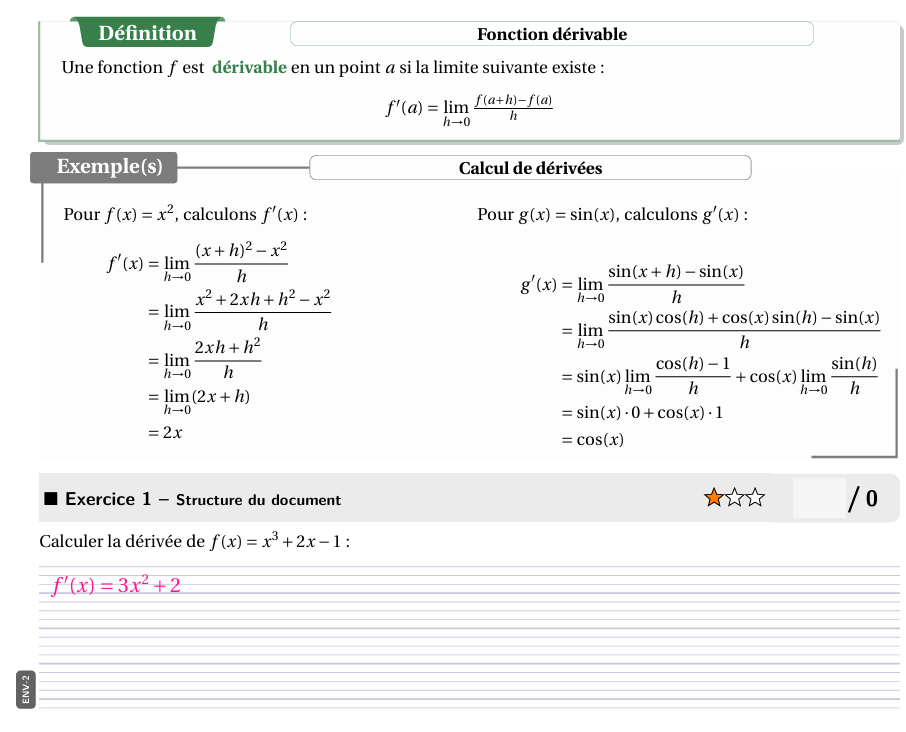
\includegraphics[width=0.75\textwidth]{sections/formattage/env/exemple-bidon.png}
        \end{center}
\end{EXO}
